\documentclass[]{article}

%&&&&&&&&&&&&&&&   PREAMBLE  %%%%%%%%%%%%%%%%

\usepackage{authblk} % Package for author affiliations
\usepackage{mathptmx} % Times New Roman text and math mode
\usepackage{color}   % For colored text
\usepackage{graphicx}
\usepackage{float}

\usepackage{abstract}



\title{Review and Analysis of Instrumentation Amplifier for Biomedical  Applications}
		
\author{JOYDEEP NATH}

\affil{Department of ECE, Assam University,\\City- Silchar, Dist-Cachar, State - Assam, India}

\begin{document}

\maketitle

%%%%%%%%%%%%%%%$  ABSTRACT   %%%%%%%%%%%%%%%%%% 

\begin{abstract}
	
		Instrumentation amplifiers(in-amp)are used in many applications,
		from motor control to data acquisition to automotive.They also play a crucial	role in biomedical applications as Bio-medical sensors detect very weak signals like Electrocardiogram (ECG), Electromyogram (EMG), Electroencephalogram (EEG) and Action potential of neurons which are on the orders of the 0.1-10mV and frequency up to 10kHz.
		To process these sensitive signals, the bio-medical device should have low noise, low offset and susceptible to 50Hz power line and other common mode disturbances.
		
	    Particularly in the context of wearable and implantable devices integrating instrumentation amplifiers(IA) with complementary metal-oxide-semiconductor (CMOS) technology for its various advantages such as scaling. Despite significant progress, challenges remain in balancing noise reduction, power optimization, and size constraints	
		
		This paper presents a comprehensive review of 20 recent research studies on the design, development and advancements in IA architectures using different typologies,though trade-offs between power consumption, accuracy, Noise Efficiency Factor(NEF) and area utilization.


\end{abstract}
\vspace{4cm}

%%%%%%%%%%%%%%%$  INTRODUCTION   %%%%%%%%%%%%%%%%%%

\section{INTRODUCTION}

		An instrumentation amplifier(IA) is a closed-loop gain block that has a differential input and an output that is single-ended with respect to a reference terminal. Unlike an OP-AMP, for which closed-loop gain is determined
		by external resistors connected between its
		inverting input and its output, an IA employs an
		internal feedback resistor network that is isolated from its
		signal input terminals. With the input signal applied across
		the two differential inputs, gain is either preset internally
		or is user set (via pins) by an internal or external gain
		resistor, which is also isolated from the signal inputs.



\begin{figure}[H]
	\centering
	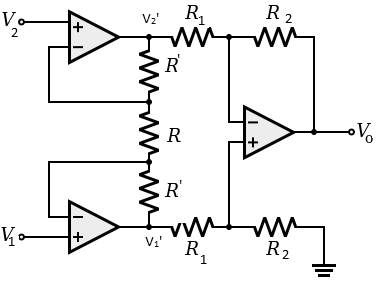
\includegraphics[width=5cm, height=5cm]{IA_DIAGRAM}
	\caption[Figure 1: Instrumentation amplifier]{}
	\label{fig:IA-CIRCUIT-DIAGRAM}
\end{figure}




\end{document}
